\section{Hadoop}

\subsection{Breve histórico}

O problema era simples: como criar um índice para uma máquina de busca de toda a Internet? Foi com esse 
desafio que Mike Cafarella e Doug Cutting resolveram desenvolver o Apache Nutch. Rapidamente o 
\textit{crawler} e a máquina de busca ficaram prontos, mas eles perceberam que a arquitetura não 
escalaria para criar um índice de mais de um bilhão de páginas da Internet. Na mesma época, a equipe 
do Google publicou um artigo que explicava a arquitetura do GFS (Google FileSystem) 
\cite{ghemawat2003google}, que era um sistema de arquivos distribuído usado em sua máquina de busca. 
Doug e Mike decidiram criar uma implementação \textit{open source} dessa arquitetura e a chamaram 
de NDFS (Nutch Distributed FileSystem).

Em 2004, a equipe do Google publicou novo artigo agora detalhando como era possível criar um índice de 
toda a Internet usando o mecanismo de processamento paralelo denominado MapReduce \cite{dean2008mapreduce}. 
Com base nesse trabalho, os desenvolvedores do Nutch migraram a maior parte de seus algoritmos para 
executar sobre o MapReduce e o NDFS. Mais tarde, Doug Cutting foi trabalhar no Yahoo! liderando uma 
equipe que construiu a nova geração de máquina de busca deles. Depois, o NDFS (posteriormente chamado
de HDFS ou \textit{Hadoop Distributed Filesystem}) e o MapReduce tornaram-se 
um projeto da Apache Software Foundation sob o nome de Apache Hadoop.

Desde então, o Hadoop tem sido usado mundialmente para processar enormes quantidades de dados. Vários 
frameworks foram construídos para executar usando a sua infraestrutura, como veremos a seguir. 
Diversos fornecedores criaram suas próprias distribuições do Hadoop, como Microsoft, IBM, EMC, Oracle e 
outras empresas especializadas como Cloudera e Hortonworks.

\subsection{Funcionamento do HDFS}

O HDFS, como mencionado acima, é um sistema de arquivos distribuídos, projetado para armazenar arquivos 
muito grandes\footnote{Atualmente há instâncias do HDFS armazenando PetaBytes de dados.} executando sobre 
hardware commodity. 

Assim como em qualquer sistema de arquivos, um arquivo é dividido em \textbf{blocos} de dados. Enquanto 
tipicamente um sistema de arquivos tradicional armazena dados em pequenos blocos (e.g. 512 bytes ou 1 kbyte), 
o HDFS usa, por padrão, blocos de 64MB. Isso torna o HDFS ineficiente para uso em arquivos muito pequenos 
e numerosos. Para garantir disponibilidade e leitura em paralelo, cada um dos blocos é replicado em um dos 
nós de um \textit{cluster} HDFS. Quando um disco ou um dos nós do \textit{cluster} falha, além do bloco 
poder ser lido de outro nó, o sistema de arquivos automaticamente recria os blocos presentes naquele disco 
em outros nós do \textit{cluster}.

\begin{figure}
	\centering
	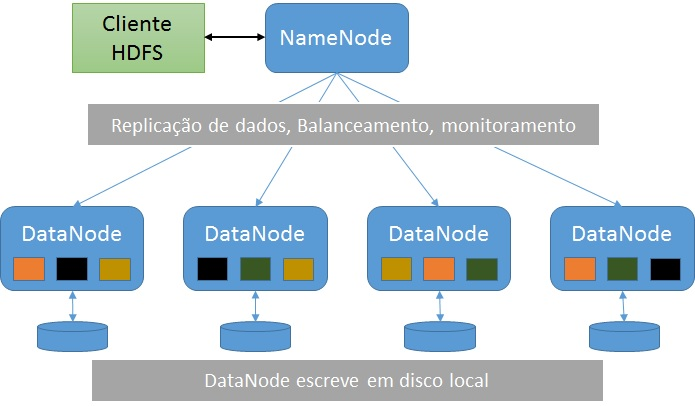
\includegraphics[width=\linewidth]{./Arquitetura_HDFS.jpg}
	\caption{Visão geral da arquitetura do HDFS}
	\label{fig:hdfs_arch}
\end{figure}

A arquitetura de um \textit{cluster} HDFS divide-se em \textit{NameNode} e \textit{DataNode}. O primeiro armazena um índice de arquivos e de seus blocos e o segundo armazena os dados (blocos). Um cliente que queira ler arquivos no HDFS, primeiro consulta o \textit{NameNode}, que então diz de quais nós do cluster os blocos serão lidos, garantindo um balanceamento de carga na leitura. Arquivos criados no HDFS só podem ser modificados anexando conteúdo no final. Não pode-se modificar blocos já escritos. A falha do \textit{DataNode} implica na indisponibilidade de todo o HDFS e, por esse motivo, é importante mantê-lo resiliente a falha com mecanismos de redundância. Uma visão geral dessa arquitetura pode ser vista na figura \ref{fig:hdfs_arch}.

\subsection{O ecossistema Hadoop}

Atualmente o Hadoop conta com um ecossistema com diversos \textit{frameworks}. Uma lista, não exaustiva, 
de alguns dos principais projetos que compõem o ecossistema pode ser vista abaixo.

\begin{itemize}
	\item Ambari: Uma ferramenta web para aprovisionamento e gerenciamento de um cluster Hadoop e de diversos de seus componentes.
	\item HBase: Um banco de dados não relacional (NoSQL) e colunar que utiliza a infraestrutura do Hadoop como mecanismo de armazenamento.
	\item Hive: Uma infraestrutura de armazém de dados com suporte a sumarização de dados e consultas.
	\item Pig: Uma linguagem de alto nível para fluxo de dados e um \textit{framework} de execução de computação distribuída. 
	\item Spark: Uma \textit{engine} rápida e de propósito geral para processamento de dados em memória baseados nos dados do HDFS. O Spark oferece um modelo de programação simples e poderoso para executar uma enorme gama de atividades como ETL, aprendizagem de máquina, processamento contínuo de dados, processamento de grafos, etc.
	\item Sqoop: uma ferramenta para transferência massiva de dados entre bancos de dados relacionais e o HDFS.
	\item Mahout: Um conjunto de bibliotecas para executar algoritmos de aprendizagem de máquina e mineração de dados. Os coordenadores do projeto decidiram mover a implementação dos algoritmos de MapReduce para o Spark.
\end{itemize}

\subsection{MapReduce}
\label{sec:mapreduce}

O Hadoop MapReduce é um \textit{framework} para facilitar a escrita de programas de computador para 
processar uma enorme quantidade de dados de forma paralela, distribuída e resiliente a falhas. Os dados 
de entrada para um \textit{job} MapReduce, por estarem armazenados no HDFS, são também processados 
de forma distribuída, aproveitando dos dados disponíveis localmente em um nó do \textit{cluster}. 
Na Figura \ref{fig:mapreduce} podemos ver um desenho esquemático de um \textit{job} MapReduce, que é, 
de forma resumida, composto por duas fases:

\begin{enumerate}
	\item \textit{Map}: quando os dados são processados e produzem saídas como tuplas no formato 
\{\emph{chave}, \emph{valor}\}; 
	\item \textit{Reduce}: quando as tuplas com mesma \emph{chave} são agrupadas para alguma atividade 
de agregação.  
\end{enumerate}

\begin{figure}
	\centering
	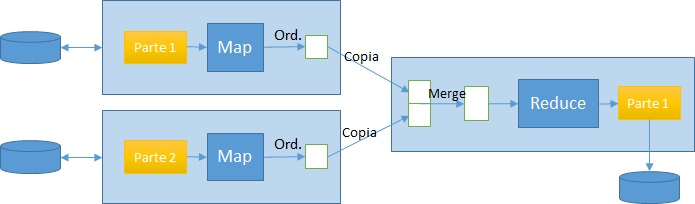
\includegraphics[width=\linewidth]{./Job_Mapreduce.jpg}
	\caption{Um \textit{job} MapReduce}
	\label{fig:mapreduce}
\end{figure}

Um exemplo bem simples para entender o MapReduce é um job para contar a ocorrência de cada palavra 
em um texto. Na fase de \textit{Map}, cada linha lida do arquivo é dividida em suas palavras que 
produzem uma saída \{PalavraA, 1\}. Note que se uma palavra aparece duas vezes na mesma linha duas 
tuplas idênticas serão produzidas. Na faze de \textit{Reduce}, as tuplas com mesma chave serão 
agrupadas e os valores $1$ serão somados. 

Em geral, o programador não precisa se preocupar com comunicação de dados, tratamento de concorrência 
e eventuais falhas em algum nó que está processando um determinado \textit{job}. Esse é um dos grandes 
diferenciais do Hadoop MapReduce. 

Uma possível solução para contagem de triângulos utilizando MapReduce, baseada na proposta feita por 
Suri e Sergei \cite{suri2011counting}, envolve o encadeamento de 3 \textit{jobs} MapReduce. O primeiro 
constrói um conjunto de todas as tríades (par de arestas que compartilham um vértice) de um grafo. Essas 
tríades, juntamente com as arestas originais são gerados como linhas, mas com um atributo identificador 
dizendo se é uma aresta original do arquivo ou se foi gerada pelo primeiro passo. Essa saída serve de 
entrada para o segundo \textit{job}, que conecta as tríades com as arestas originais, formando os 
triângulos. Por fim, o terceiro \textit{job} conta o número de triângulos gerados pelo passo anterior. 
Vamos olhar um exemplo para melhor entendimento.  

Dada o grafo não direcionado de entrada descrita na tabela \ref{grafoExemplo}, onde os números identificam 
os nós e cada linha uma aresta que liga esses vértices, podemos identificar 3 triângulos: 
(Bernardo, Chico, Renato), (Renato, Chico, Roberto) e (André, Bianca, Marcelo).

\begin{table}[]
\centering
\caption{Exemplo de grafo de entrada.}
\label{grafoExemplo}
\begin{tabular}{cc}
\hline
{\bf Origem} & {\bf Destino} \\ \hline
André        & Bernardo      \\ \hline
André        & Marcelo       \\ \hline
André        & Bianca        \\ \hline
Bernardo     & Chico         \\ \hline
Bernardo     & Renato        \\ \hline
Chico        & Renato        \\ \hline
Chico        & Roberto       \\ \hline
Chico        & Livia         \\ \hline
Marcelo      & Bianca        \\ \hline
Roberto      & Renato        \\ \hline      
\end{tabular}
\end{table}

Após a etapa de \textit{Map} do primeiro \textit{job}, são gerados um conjunto de 
\{\textit{chave}, \textit{valor}\} conforme a tabela \ref{map1}. Note que a chave é escolhida como 
o vértice de menor valor.

\begin{table}[]
\centering
\caption{Resultado da etapa de Map do primeiro \textit{Job}.}
\label{map1}
\begin{tabular}{cc}

\hline
{\bf Chave} & {\bf Valor (arest)}      \\ \hline
André       & André, Marcelo   \\ \hline
André       & André, Bianca    \\ \hline
André       & André, Bernardo  \\ \hline
Marcelo     & Marcelo, Bianca  \\ \hline
Bernardo    & Bernardo, Chico  \\ \hline
Bernardo    & Bernardo, Renato \\ \hline
Chico       & Chico, Roberto   \\ \hline
Chico       & Chico, Livia     \\ \hline
Chico       & Chico, Renato    \\ \hline
Roberto     & Roberto, Renato  \\ \hline     
\end{tabular}
\end{table}

A etapa de \textit{Reduce} do primeiro \textit{job} é a mais importante. Nessa etapa, para cada chave 
da Tabela \ref{map1}, são gerados as arestas originais (valor na tabela) bem como as tríades baseadas 
nessas arestas. O resultado, já ordenado, pode ser visto na tabela \ref{reduce1}.

\begin{table}[]
\centering
\caption{Resultado da etapa de Reduce do primeiro \textit{Job}.}
\label{reduce1}
\begin{tabular}{ccc}
\hline
{\bf Chave}                                                    & {\bf Gerado} & {\bf Tríades}                                                                         \\ \hline
\begin{tabular}[c]{@{}c@{}}André,\\   Bernardo\end{tabular}    & 0            &                                                                                       \\ \hline
\begin{tabular}[c]{@{}c@{}}André,\\   Marcelo\end{tabular}     & 0            &                                                                                       \\ \hline
\begin{tabular}[c]{@{}c@{}}André,\\   Bianca\end{tabular}      & 0            &                                                                                       \\ \hline
\begin{tabular}[c]{@{}c@{}}Bernardo,\\   Chico\end{tabular}    & 0            &                                                                                       \\ \hline
\begin{tabular}[c]{@{}c@{}}Bernardo,\\   Bianca\end{tabular}   & 1            & \begin{tabular}[c]{@{}c@{}}\{André, Bernardo\}, \{André,\\   Bianca\}\end{tabular}    \\ \hline
\begin{tabular}[c]{@{}c@{}}Bernardo,\\   Renato\end{tabular}   & 0            &                                                                                       \\ \hline
\begin{tabular}[c]{@{}c@{}}Bernardo, \\   Marcelo\end{tabular} & 1            & \begin{tabular}[c]{@{}c@{}}\{André, Bernardo\}, \{André,\\   Marcelo\}\end{tabular}   \\ \hline
\begin{tabular}[c]{@{}c@{}}Chico,\\   Livia\end{tabular}       & 0            &                                                                                       \\ \hline
\begin{tabular}[c]{@{}c@{}}Chico,\\   Roberto\end{tabular}     & 0            &                                                                                       \\ \hline
\begin{tabular}[c]{@{}c@{}}Chico,\\   Renato\end{tabular}      & 1            & \begin{tabular}[c]{@{}c@{}}\{Bernardo, Chico\}, \{Bernardo,\\   Renato\}\end{tabular} \\ \hline
\begin{tabular}[c]{@{}c@{}}Chico,\\   Renato\end{tabular}      & 0            &                                                                                       \\ \hline
\begin{tabular}[c]{@{}c@{}}Livia,\\   Roberto\end{tabular}     & 1            & \{Chico, Livia\}, \{Chico, Roberto\}                                                  \\ \hline
\begin{tabular}[c]{@{}c@{}}Livia,\\   Renato\end{tabular}      & 1            & \{Chico, Livia\}, \{Chico, Renato\}                                                   \\ \hline
\begin{tabular}[c]{@{}c@{}}Marcelo,\\   Bianca\end{tabular}    & 1            & \begin{tabular}[c]{@{}c@{}}\{André, Marcelo\}, \{André,\\   Bianca\}\end{tabular}     \\ \hline
\begin{tabular}[c]{@{}c@{}}Marcelo,\\   Bianca\end{tabular}    & 0            &                                                                                       \\ \hline
\begin{tabular}[c]{@{}c@{}}Roberto,\\   Renato\end{tabular}    & 1            & \begin{tabular}[c]{@{}c@{}}\{Chico, Roberto\}, \{Chico,\\   Renato\}\end{tabular}     \\ \hline
\begin{tabular}[c]{@{}c@{}}Roberto,\\   Renato\end{tabular}    & 0            &                                                                                       \\ \hline
\end{tabular}
\end{table}

O segundo \textit{job} tem apenas a etapa de \textit{Reduce} e toma de entrada o resultado produzido na 
Tabela \ref{reduce1}. Para cada grupo de chaves (arestas), é verificado se há uma aresta original 
(Gerado = 0). Se sim, é verificada em quantas tríades essa aresta fecha um triângulo, emitindo uma 
contagem parcial para cada chave. Pelo nosso exemplo, podemos ver que isso ocorre nas chaves 
(Chico, Renato), (Lívia, Renato) e (Marcelo, Bianca), totalizando nossos 3 triângulos.

A última etapa (terceiro \textit{Job}) é uma tarefa trivial de somar as contagens parciais emitidas 
pelo passo anterior.

\subsection{Hive}

O Hadoop MapReduce, como descrito anteriormente na Seção \ref{sec:mapreduce}, é um framework para ser 
utilizado e desenvolvido em uma linguagem de programação, e.g. Java, com as complexidades inerentes de 
um desenvolvimento de software em linguagens de computação. Assim surgiu rapidamente a necessidade de 
especificação de programas MapReduce em linguagens declarativas de alto nível.

O Hive \cite{thusoo2009hive} é então uma das iniciativas neste sentido, sendo uma especificação de 
\textit{jobs} MapReduce em linguagem similar ao SQL: o HiveQL. O Hive foi inicialmente desenvolvido 
pelo Facebook e atualmente seus principais contribuidores são o próprio Facebook e o Netflix.

O Hive entende arquivos do HDFS como tabelas com estrutura, de forma similar a um SGBD. Entretanto, 
nenhuma estrutura adicional de SGBD é criada pelo Hive, exceto os metadados sobre o formato dos arquivos 
em tabelas. No HiveQL há uma linguagem de definição destes formatos.

Como um exemplo, vamos imaginar que temos um arquivo contendo os dados do Twitter no HDFS contendo 
os dados da tabela do twitter descrita na Seção \ref{sec:relacional} com atributos \textit{follower} e
\textit{followee}, ou seja, um arquivo texto em formato CSV contendo dois números inteiros (delimitados
por vírgula). O comando HiveQL abaixo cria os metadados para a tabela Twitter a partir deste arquivo.

\begin{verbatim}
CREATE TABLE twitter (follower INT, followee INT);
LOAD DATA INPATH '/input/twitter' OVERWRITE INTO TABLE twitter;
\end{verbatim}

Embora o HiveQL não implemente a linguagem SQL em todas as suas funcionalidades, a consulta da
Seção \ref{sec:relacional} que resolve o problema da contagem dos triângulos pode ser aplicada
diretamente no console do Hive.

É importante notar que o Hive interpreta o SQL e gera \textit{jobs} MapReduce em Java, que são
compilados e executados sob demanda.

\subsection{Pig}

De forma similar ao Hive, o Yahoo! criou o Pig \cite{olston2008pig} em 2006 e o moveu como um projeto 
para o Hadoop em 2007, com o intuito de simplificar o desenvolvimento de \textit{jobs} MapReduce 
através de uma linguagem procedural de alto nível (Pig Latin).

O Pig Latin, diferentemente do HiveQL, é uma linguagem procedural e não declarativa. É possível 
efetuar atribuições e manipulação de variáveis intermediárias. Em geral, cada comando PigLatin
corresponde a um operador da álgebra relacional.

O exemplo abaixo mostra a declaração da tabela do Twitter na linguagem Pig Latin.

\begin{verbatim}
Twitter = LOAD '/input/twitter' USING PigStorage(',') 
  AS (follower: int, followee: int);
\end{verbatim}

Note que, diferentemente do Hive, o Pig Lating cria a tabela Twitter e ao mesmo tempo instancia 
a mesma lendo do arquivo de input com o formato especificado.

O código abaixo executa a contagem dos triângulos, uma vez mapeada a tabela Twitter.

\begin{verbatim}
Twitter_1 = LOAD '/input/twitter' USING PigStorage(' ') 
  AS (follower:int, followee:int);
Twitter_2 = LOAD '/input/twitter' USING PigStorage(' ') 
  AS (follower:int, followee:int);
Twitter_3 = LOAD '/input/twitter' USING PigStorage(' ') 
  AS (follower:int, followee:int);

Twitter_SelfJoin = JOIN Twitter_1 by $1, 
                        Twitter_2 by $0;

Twitter_FullJoin = JOIN Twitter_3 by ($1, $0), 
                        Twitter_SelfJoin by ($0, $3);

Triangles = FILTER Twitter_FullJoin 
  BY ($0 < $1 AND $1 < $3) OR ($0 > $1 AND $1 > $3);

Triangles_Grp = GROUP Triangles ALL;
Triangles_Cnt = FOREACH Triangles_Grp GENERATE COUNT(Triangles);

DUMP Triangles_Cnt;
\end{verbatim}

As três primeiras linhas atribuem as tabelas Twitter\_1, Twitter\_2 e Twitter\_3. Esta atribuição 
em três tabelas não deveria ser necessária, mas na versão do Pig (antiga) em que criamos e executamos
este código não era possível fazer uma junção da tabela com ela mesma (\emph{self join}).

As próximas duas linhas executam as duas junções; a próxima, um filtro que elimina as duplicatas;
e as duas penúltimas executam um agrupamento para contagem. A última linha imprime o valor final.
Somente a partir de um comando DUMP que o Pig começa a construir os \textit{jobs} MapReduce, compilar
e executá-los.

\section{Apache Spark}

O Apache Spark é uma plataforma para computação distribuída que foi projetada para ser de propósito 
geral e muito eficiente \cite{zaharia2012resilient, karau2015learning}. A principal diferença em 
relação ao MapReduce é que toda a computação é feita e armazenada em memória, sem necessidade de salvar 
em disco resultados intermediários. 

A unidade básica de dados do Spark é o \textit{Resilient Distributed Dataset} (RDD). O conceito é 
semelhante ao bloco de dados do HDFS, mas trata-se de coleções de dados que estão na memória RAM dos 
nós do \textit{cluster}. Na prática, o Spark carrega os dados de um bloco do HDFS na memória RAM do nó 
em que o bloco está. Os programas Spark fazem dois tipos de operação com um RDD:

\begin{itemize}
	\item \textbf{Transformações}: Transformam um RDD em outro RDD. Entre as transformações mais 
comuns podemos encontrar as operações de \textit{Map} e \textit{ReduceByKey} (mesmo conceito do MapReduce), 
ordenação e operações de conjuntos, como união, interseção e diferença.
	\item \textbf{Ações}: Produzem algum resultado a partir de um RDD. Ações típicas consistem em 
enumerar alguma quantidade de itens de um RDD, contar e somar. 
\end{itemize}

O Spark utiliza o conceito de \emph{execução preguiçosa}, para que só quando realmente um resultado 
tenha de ser produzido (uma \textbf{ação} é executada), e toda a sequência de passos necessária é 
conhecida, o Spark realmente lê os dados e faz cálculos na memória. Com isso, o motor de execução do 
Spark consegue otimizar tudo que será executado, escolhendo os melhores nós, a melhor sequência, etc.

O Apache Spark também vem com um conjunto de bibliotecas com algoritmos para aprendizado de máquina, 
grafos, fluxo contínuo de dados e SQL. Algumas dessas vermos a seguir.

\subsection{Utilizando o console python}
O Apache Spark possui consoles iterativos nas linguagens Python e Scala e seus \textit{jobs} podem 
ser submetidos em batch também em Java. A API do Spark é acessada a partir de um objeto central 
denominado \texttt{SparkContext}. Esse objeto contém a conexão com uma instância do cluster e a partir 
dele todos os outros objetos e métodos são acessados. Ao se iniciar um console do Spark, o objeto já 
está automaticamente disponível através da variável \texttt{sc}. Para compreender a simplicidade 
do modelo de programação do Spark, o trecho de código abaixo lê um arquivo txt e faz a contagem de 
ocorrência das palavras.

\begin{lstlisting}[style=MyPythonStyle]
#produz um RDD onde cada item e uma linha do arquivo texto
arquivo = sc.textFile('hdfs://servidor:10001/arquivo.txt') 

#para cada linha produz N itens no novo RDD, uma para cada palavra.
palavras = arquivo.flatMap(lambda linha : linha.split(' ')) 

#cria novo RDD com tuplas do formato (palavra, 1)
palavrasCV = palavras.map(lambda palavra : (palavra, 1)) 

#executa o Reduce usando a funcaoo add para os valores das tuplas.
contagemPalafras = palavrasCV.reduceByKey(add) 

#somente nesse comando toda a computacaoo e feita de forma otimizada.
contagemPalavras.collect() 
\end{lstlisting}

Para resolver o problema de contagem de triângulos utilizando o Spark, a ideia é semelhante à usada com 
o modelo do MapReduce.

\subsection{Spark SQL}
O Spark SQL \cite{xin2013shark, armbrust2015spark}, anteriormente chamado de Shark, é um módulo do Apache 
Spark para processamento de dados estruturados (relacionais). Ele utiliza uma abstração denominada 
\emph{DataFrame}, e também serve como uma máquina de execução de consultas distribuídas baseada em SQL. 

Um \emph{DataFrame} do Spark SQL tem as mesmas características de um \emph{DataFrame} em R ou em 
Pandas (Python), e pode ser criado a partir de diversas fontes de dados, como um arquivo JSON, um 
arquivo texto, um RDD do Spark, uma tabela do Hive, ou qualquer fonte que possua um driver JDBC. 
O esquema de dados de um \emph{DataFrame} pode ser inferido através de reflexão ou programaticamente. 

O trecho de código abaixo mostra como executar a contagem de triângulos utilizando o SQL proposto na 
seção \ref{sec:triangulos}.

\begin{lstlisting}[style=MyPythonStyle]
# Importa os modulos e cria o contexto
from pyspark.sql import SQLContext, Row
sqlContext = SQLContext(sc)

# Carrega o arquivo de arestas para um RDD
linhas = sc.textFile("hdfs://servidor:10001/data/triangles/twitter_combined.txt")
partes = linhas.map(lambda l: l.split())
arestas = partes.map(lambda p: Row(follower=int(p[0]), followee=int(p[1])))

# Infere o schema e registra o DataFrame como tabela
schemaWiki = sqlContext.createDataFrame(arestas)
schemaWiki.registerTempTable("arestas")

# Executa o SQL
triangulos = sqlContext.sql("SELECT count(*) FROM arestas R, arestas S, arestas T " +
    " WHERE R.follower = S.followee AND S.follower = T.followee AND T.follower = R.followee")
print triangulos.collect()
\end{lstlisting}


\subsection{Spark GraphX}

O Spark GraphX é um novo módulo do Apache Spark que fornece um conjunto de abstrações e ferramentas 
para processamento paralelo de algoritmos em grafos \cite{xin2013graphx}. Nas abstrações de 
vértices e arestas é possível 
incluir propriedades, como pesos, capacidades máximas e mínimas; ou qualquer outra propriedade que 
seja relevante para modelar um problema. 

O Spark GraphX possui um conjunto de operações essenciais para diversos algoritmos de análise de grafos, 
como operações em paralelo sobre os vértices/arestas dos grafos, obtenção de subgrafos, inversão de 
arestas e agregação de vizinhos. Esse último, por exemplo, pode ser usado para calcular o grau de cada 
vértice de um grafo. Mais detalhes desse módulo podem ser obtidos na documentação oficial do produto 
\footnote{http://spark.apache.org/docs/latest/graphx-programming-guide.html}. 

Como é recente seu desenvolvimento, ainda são poucos os algoritmos implementados e a única linguagem 
suportada é o Scala. Atualmente conta com algoritmos de PageRanki \cite{brin2012reprint}, identificação 
de componentes conectados e contagem de triângulos, que demonstramos o uso no trecho de código abaixo. 
Comparado com as estratégias de MapReduce, a contagem de triângulos utilizando Spark GraphX é de 
várias ordens de grandeza mais rápido e eficiente em consumo de memória. 

\begin{lstlisting}[style=MyPythonStyle]
# Carrega o grafo a partir de um arquivo cujas linhas sao pares de identificadores dos nos, definindo uma aresta
val graph = GraphLoader.edgeListFile(sc, "graphx/data/followers.txt", true).partitionBy(PartitionStrategy.RandomVertexCut)

# conta o numero de triangulos
val triCounts = graph.triangleCount().vertices

# imprime o resultado
println(triCounts.mkString("\n"))
\end{lstlisting}
